\index{Model Build ! visualization}
The current version of \mut\ writes Tecplot-compatible output files that can be visualized to check the following attributes for \gwf, \swf\ and \cln\ model domains:
\begin{itemize}
  \item Finite-element mesh and \mfus\ cell locations derived from it
  \item Material properties
  \item Initial conditions
  \item Boundary conditions (if specified)
\end{itemize}

A \tecplot\ layout file, \texttt{\_build.lay}, has been created for each verification example and  provides a quick way to view the results of the model build.
We will demonstrate some basic concepts using the verification example \texttt{1\_VSF\_Column}, which has a \gwf\ domain defined by a simple 1D column mesh with boundary conditions assigned to the  top and bottom cells.

To load \texttt{\_build.lay} in \tecplot\ first navigate to the folder in File Explorer (e.g.\ \texttt{C:$\backslash$Work$\backslash$Examples$\backslash$\-1\_VSF\_Column}) then highlight the path in File Explorer:

        
\includegraphics[width=0.4\textwidth]{3_12_HighlightPath}

Replace the existing path with the string 'cmd':

        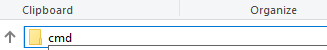
\includegraphics[width=0.5\textwidth]{3_4_cmd}

Press Enter/Return. A command prompt window rooted at the input folder should appear. To start \tecplot\, type:
        \begin{verbatim}
            tec360
        \end{verbatim}

Choose 'Open Layout' to open a file selection dialogue:

        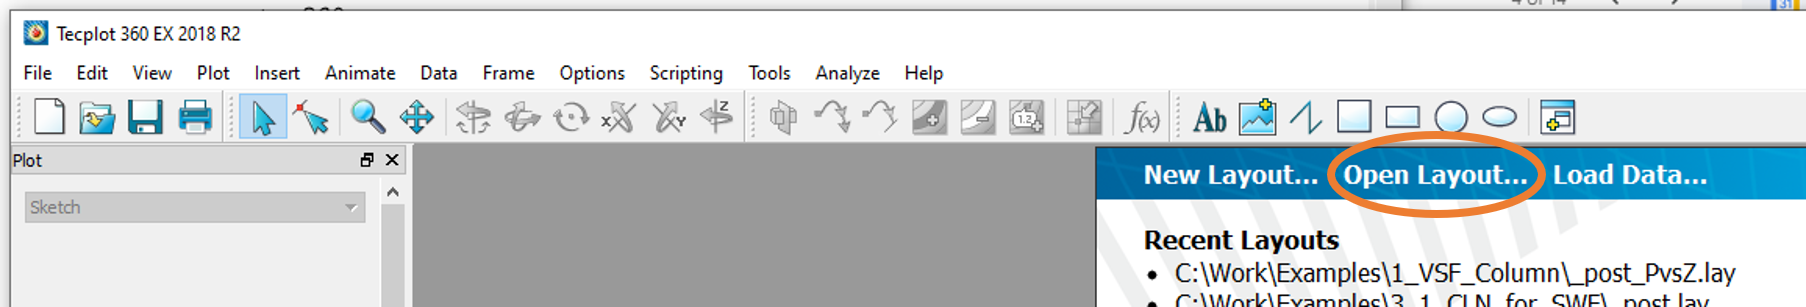
\includegraphics[width=\textwidth]{3_12_OpenLayout}

Select and open the file \texttt{\_build.lay}:

        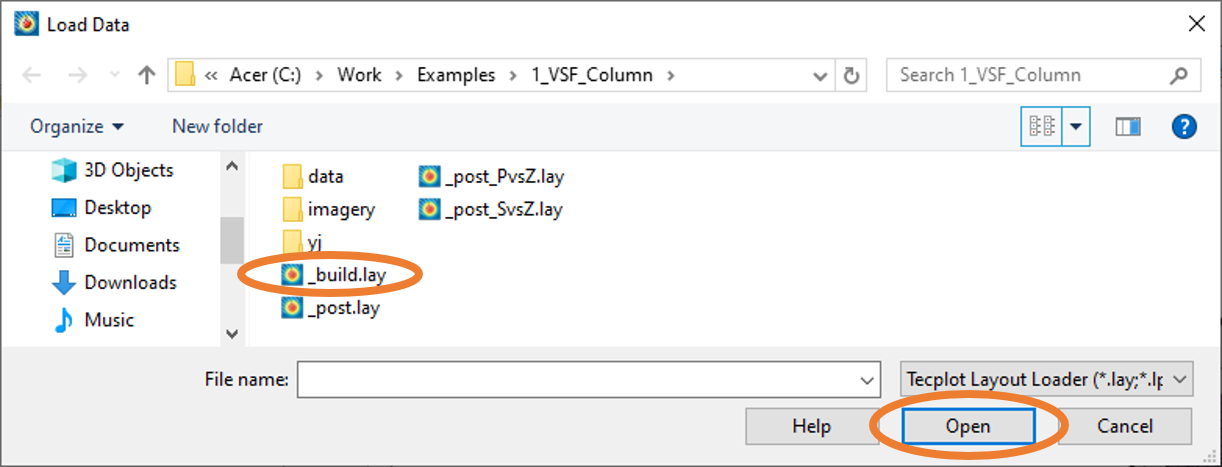
\includegraphics[width=.7\textwidth]{3_13_LayoutFiles}

You should now see the following 3D viualization of the example:

        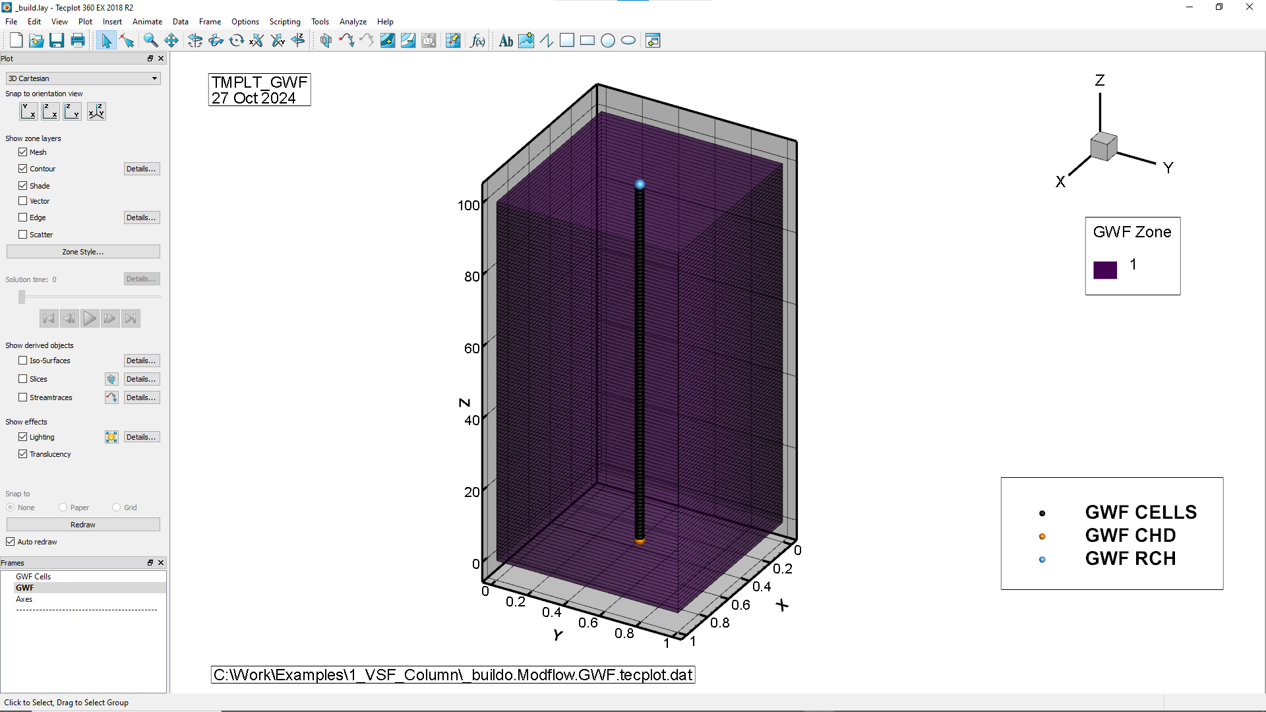
\includegraphics[width=\textwidth]{3_14_BuildLay1DColumn}

\index{\tecplot\ ! frame order}There are 4 Tecplot 'frames' that make up this image.  Each frame can house it's own data for plotting, and have unique settings for visualization.  The 'Frames' window at the bottom left corner shows the frame names and plotting order:

        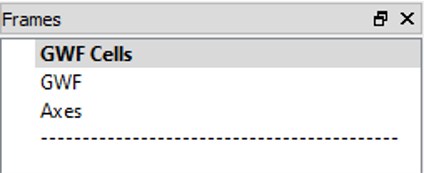
\includegraphics[width=.3\textwidth]{3_15_Frames}

The frame at the front, called \textbf{GWF Cells}, is at the top of the list, and the bold font indicates it is the currently active frame.

The frame at the bottom, indicated by the dashed line, is a special frame we will refer to as the {\sf background}.  The contents of any frame above it may be partly or completely visible, depending on which other frames are in front of it.  Move the {\sf background} to the front by right-clicking on the name and selecting 'Bring to front'.

        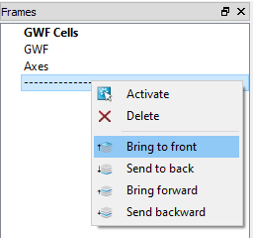
\includegraphics[width=.215\textwidth]{3_16_BringToFront}

You should now see an empty white \tecplot\ image. Right-click on the {\sf GWF} frame and bring it to the front to see it in isolation.

        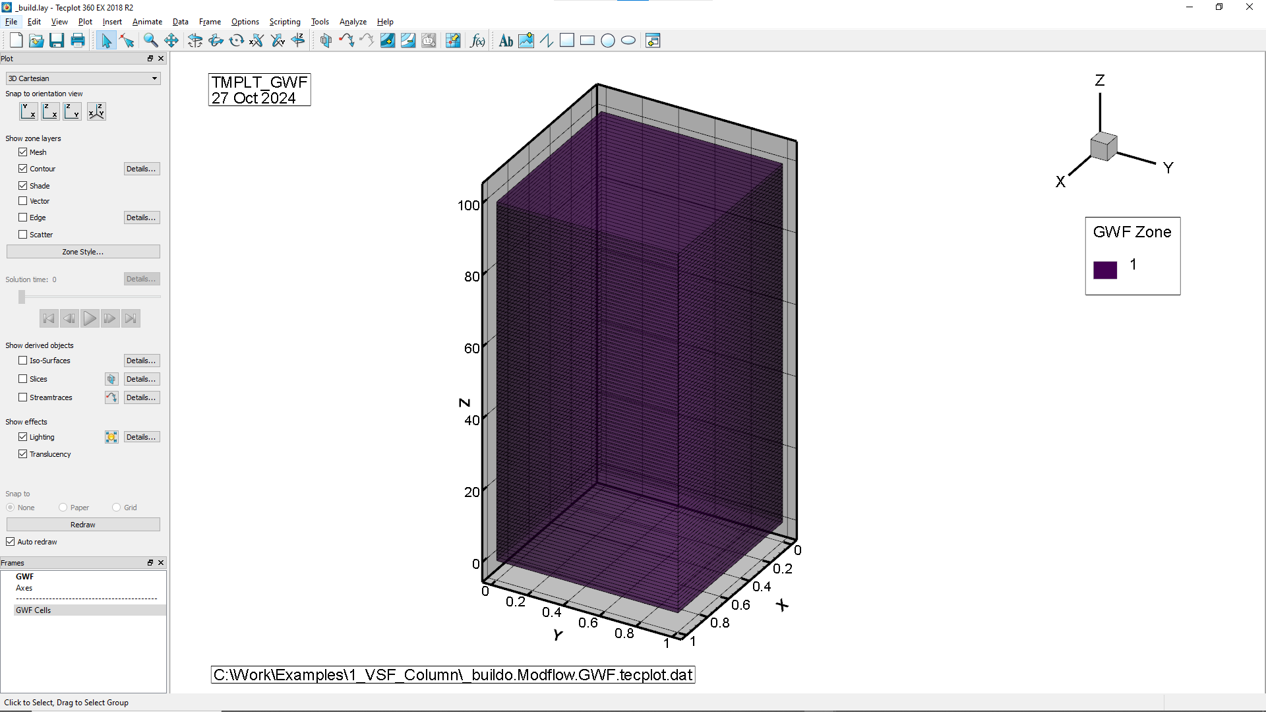
\includegraphics[width=.9\textwidth]{3_16b_GWFOnly}

Every frame below the {\sf background} frame is now invisible.

\index{\gwf\ Domain ! {\tt \_build.lay} ! {\sf GWF} frame}
The {\sf GWF} frame has the following contents:
\begin{itemize}
  \item The finite-element mesh is shown by the translucent blue-shaded volume and wireframe block elements.
  \item The names of the data files loaded into the frame are shown at the bottom left corner.
  \item The data set title and current date (on the day the file was loaded) are shown at the top left corner.  The data set title 'TMPLT\_GWF' indicates that this is the \gwf\ domain mesh that was created from the template mesh.
  \item The contouring legend, showing there is one \gwf\ zone called {\sf Zone 1}, is shown at the middle right side.
  \item The 3D orientation axis is shown at the top right corner.
\end{itemize}

Right-click on the {\sf Axes} frame and bring it to the front.

        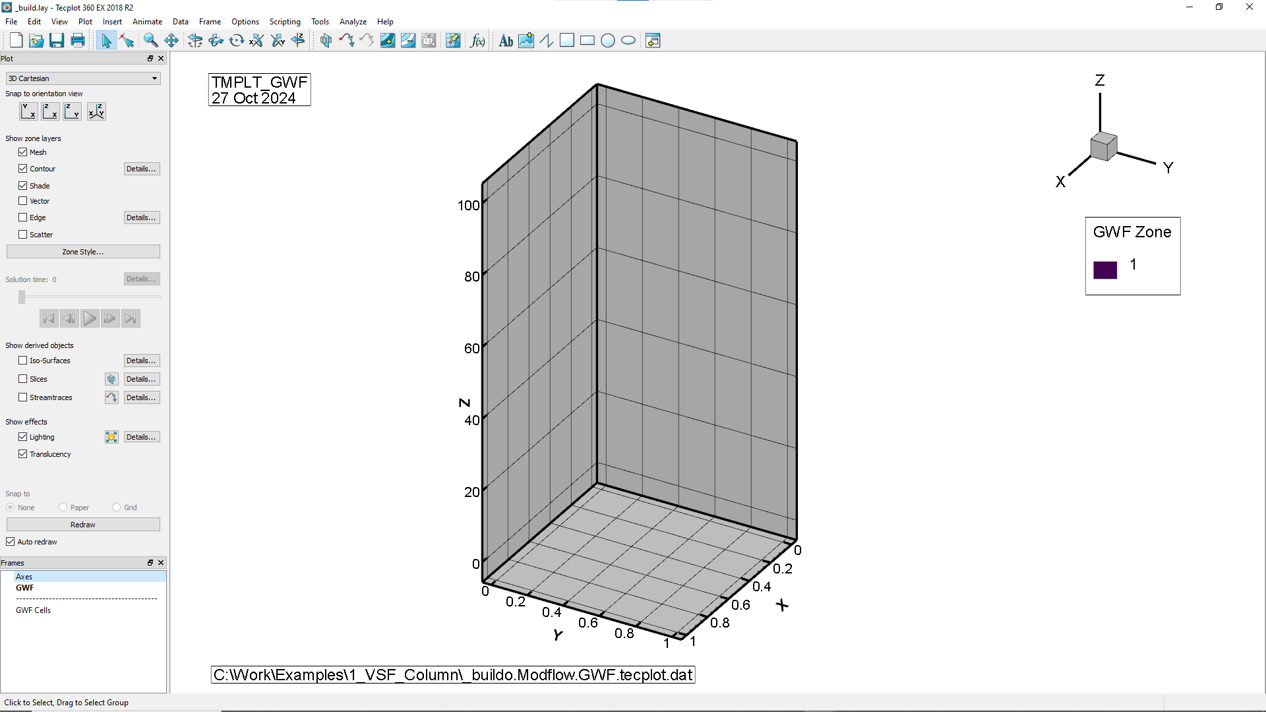
\includegraphics[width=.76\textwidth]{3_17_Axes}

Some of the contents of the {\sf GWF} frame are still visible but the finite-element mesh is obscured by the axes.  Right-click on the {\sf GWF} frame and bring it to the front.

        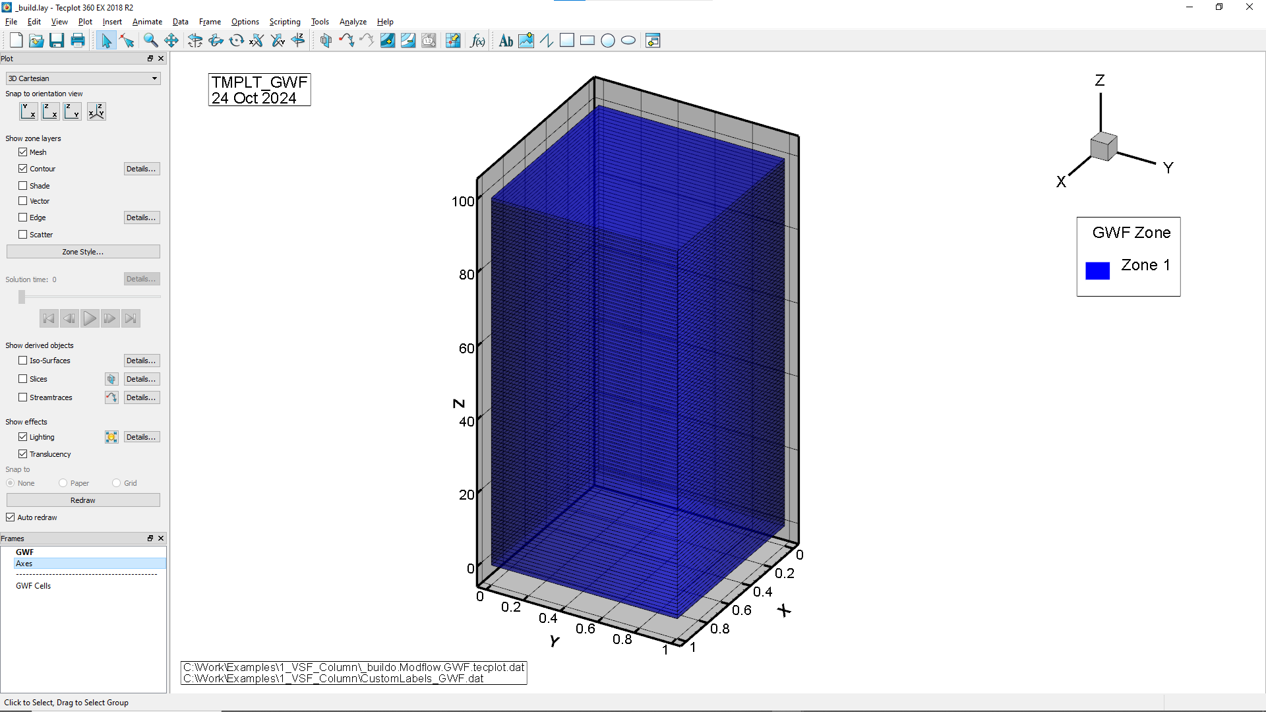
\includegraphics[width=.76\textwidth]{3_18_GWFBeforeAxes}

  The menu option {\sf Data$\backslash$Data Set Info...}(shown below left), brings up the {\sf Data Set Information} dialogue(shown below right):

        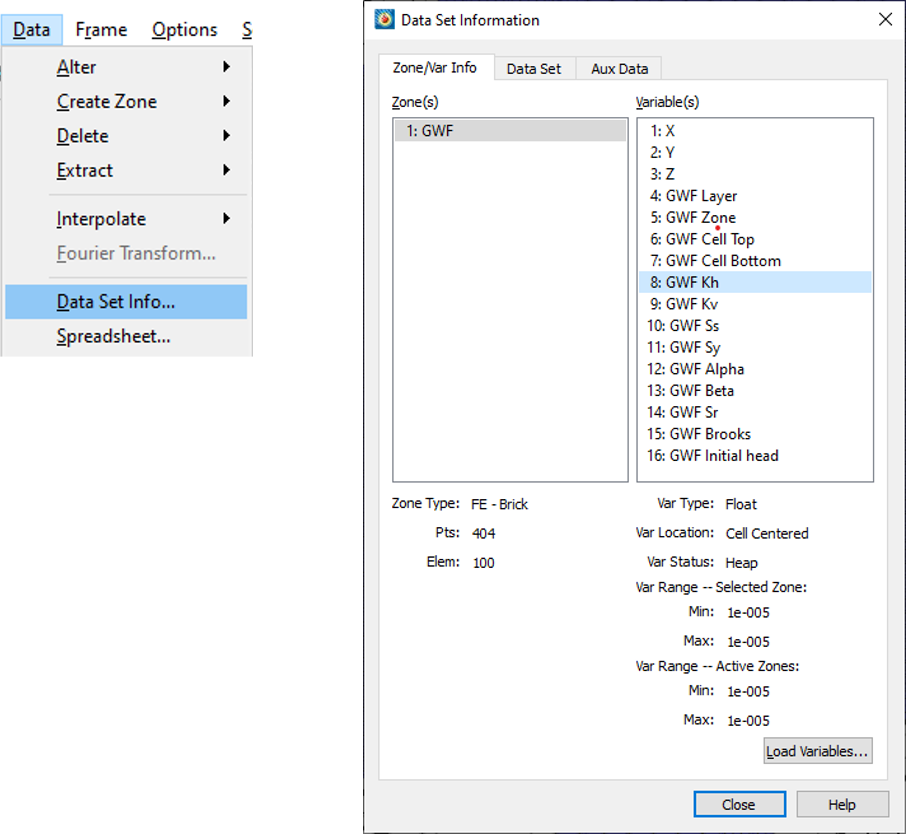
\includegraphics[width=.75\textwidth]{3_19_DataSetInfo}

The currently active frame title \gwf\ is shown in the {\sf Zone(s)} field, while the data set variables are listed in the {\sf Variable(s)} field. The variables include the $xyz$ coordinates of the {\sf TMPLT\_GWF} mesh nodes, followed by the Layer and Zone numbers assigned to the {\sf TMPLT\_GWF} mesh elements.  The remainder of the list shows the \mfus\ cell properties that were defined during the model build. The {\sf Var--Range Selected Zone:} area shows the variable {\sf Min:} and {\sf Max:} values for the currently chosen (highlighted) zone and variable (currently \gwf\ and {\sf GWF Kh} respectively).\index{\tecplot\ ! data set information}


\index{\tecplot\ ! probe tool} The \tecplot\ Probe Tool 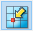
\includegraphics{ProbeToolButton} is used to to probe for values of the dataset's variables at a particular point. When selected, the mouse cursor changes to a modified cross-hair which indicates the Probe Tool is active. To obtain {\it interpolated} values of the dataset variables at the specified location, click at any point in the data region. 

Shown below are the results of probing the top cell of the \gwf\ domain:

        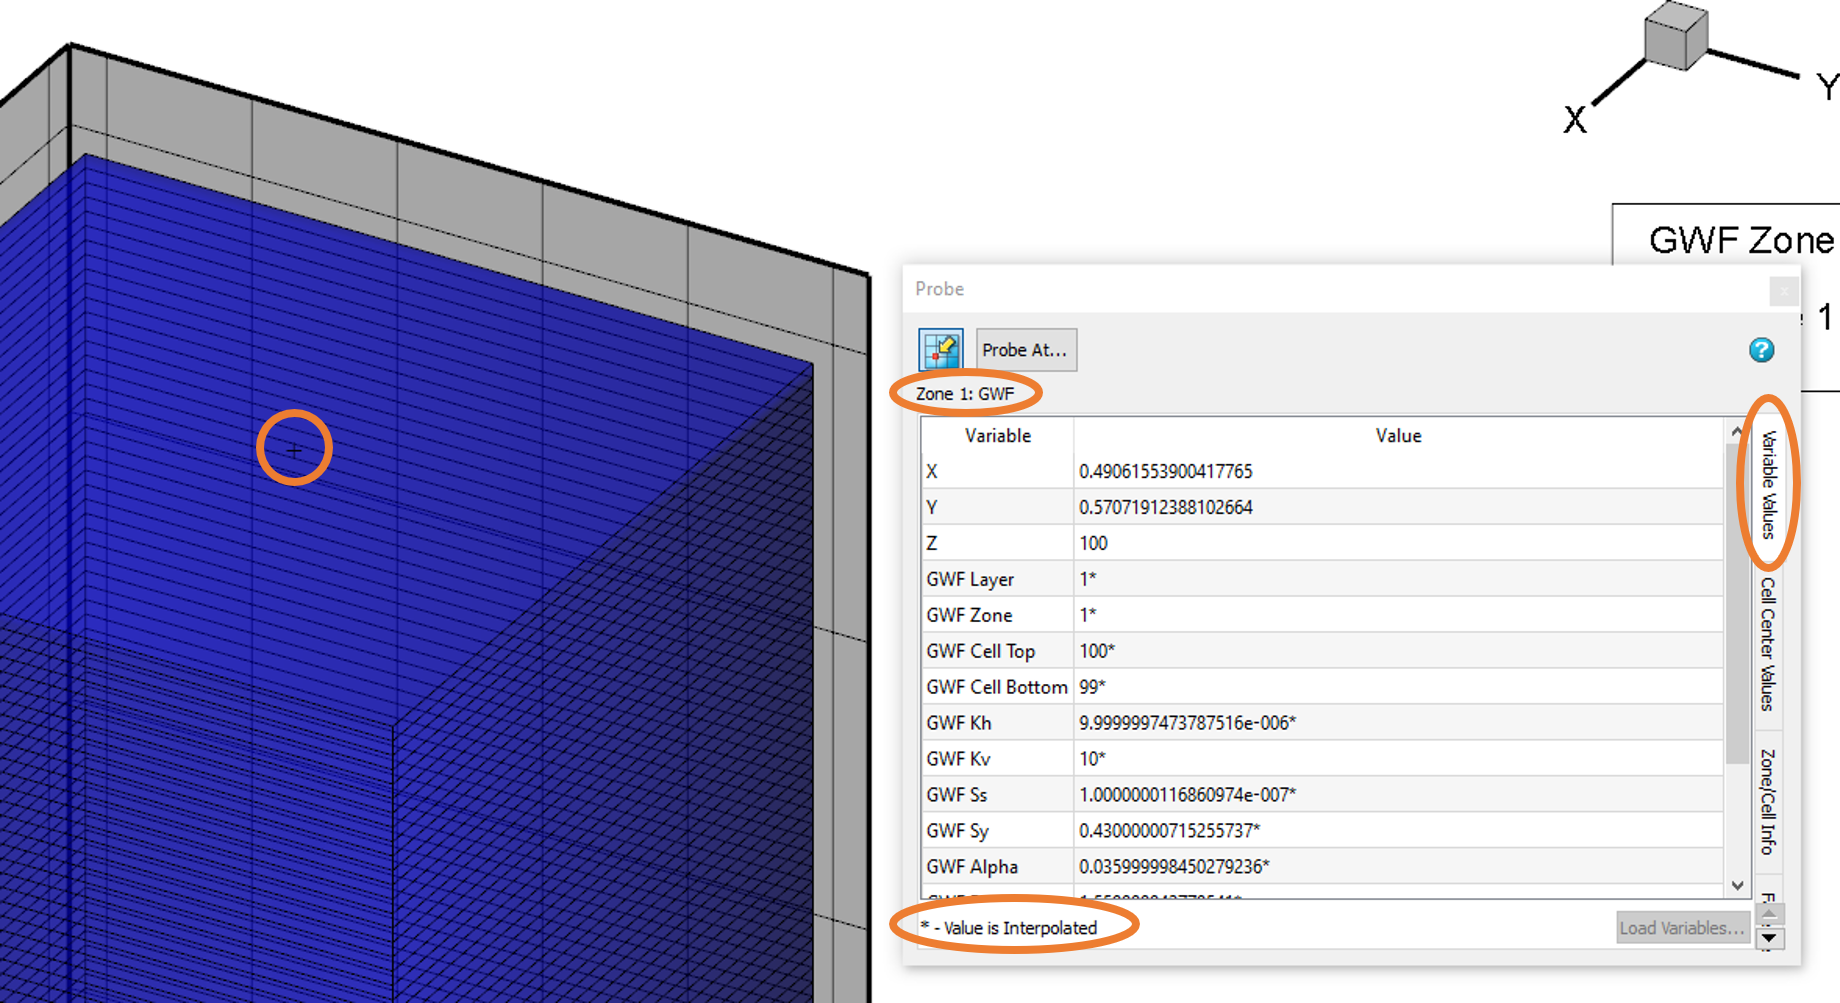
\includegraphics[width=.9\textwidth]{3_20_ProbeTool}

The probe location is indicated by the small '+' sign in the top cell (left orange circle).  This opens the {\sf Probe} dialogue which shows the zone probed ({\sf Zone 1: GWF}), and a table of  Variable names and values.

It is important to understand that in \tecplot\ nomenclature, the {\sf Variable Values} tab refers to values assigned to {\sf TMPLT\_GWF} mesh nodes, while the {\sf Cell Centred Values} tab ({\em Not to be confused with \mf\ cells!}) refers to values assigned to {\sf TMPLT\_GWF} mesh elements.

If the mesh-centred control volume approach is used, as is the case for this example, then \mf\ cell locations align with {\sf TMPLT\_GWF} mesh element centroids, and all values except the $XYZ$ coordinates (which are defined at {\sf TMPLT\_GWF} mesh nodes)  are interpolated (as indicated by an asterisk {\sf *} appended to the value}).  The $XYZ$ coordinates show the exact location of the small '+' sign.

If we select the {\sf Cell Centred Values} tab, the {\sf Probe} output looks like this:

        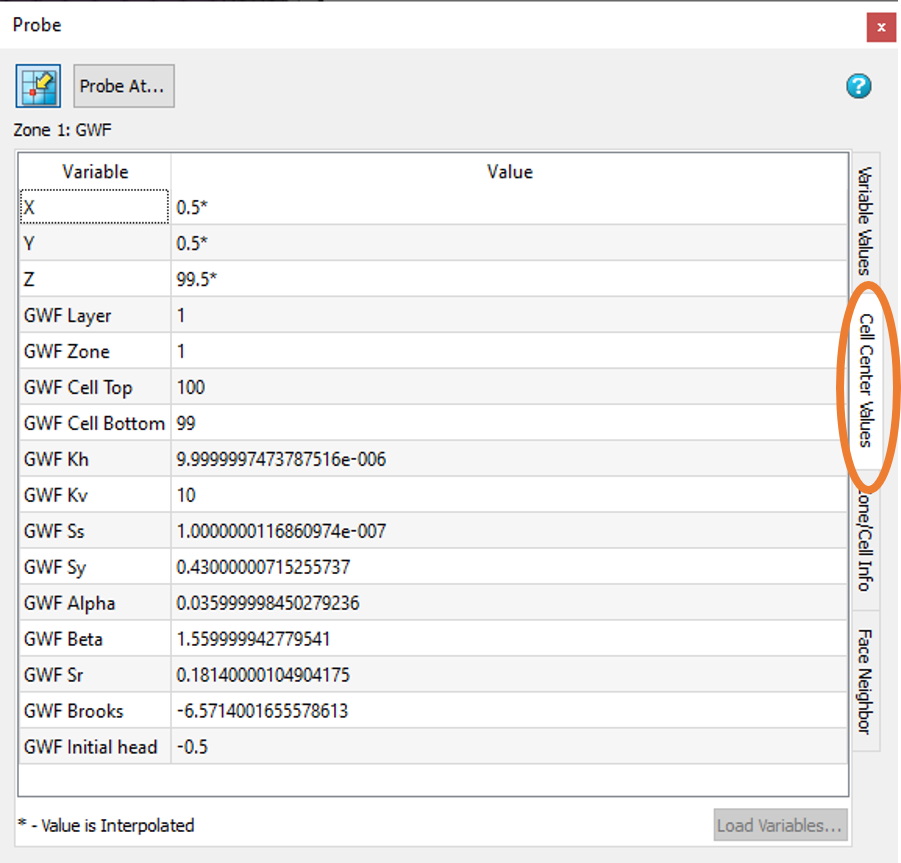
\includegraphics[width=.5\textwidth]{3_20_ProbeToolCellCentred}

Now the $XYZ$ coordinates are interpolated and show the approximate {\sf TMPLT\_GWF} mesh element centroid location, while for all other variables, exact values (i.e.\ what was input) are shown.

If the node-centred control volume approach is used, as is the case for the \texttt{6\_Abdul\_Prism\_Cell\_nc} example, then \mf\ cell locations align with {\sf TMPLT\_GWF} mesh nodes, and no variable values are interpolated when the {\sf Cell Centred Values} tab is selected.

        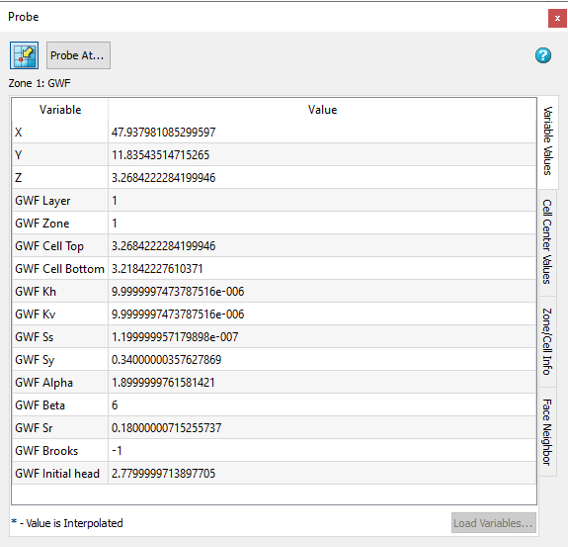
\includegraphics[width=.5\textwidth]{3_21_ProbeToolAbdul_nc}

Bring the {\sf GWF Cells} frame to the front, and send the {\sf GWF} frame to the back.

        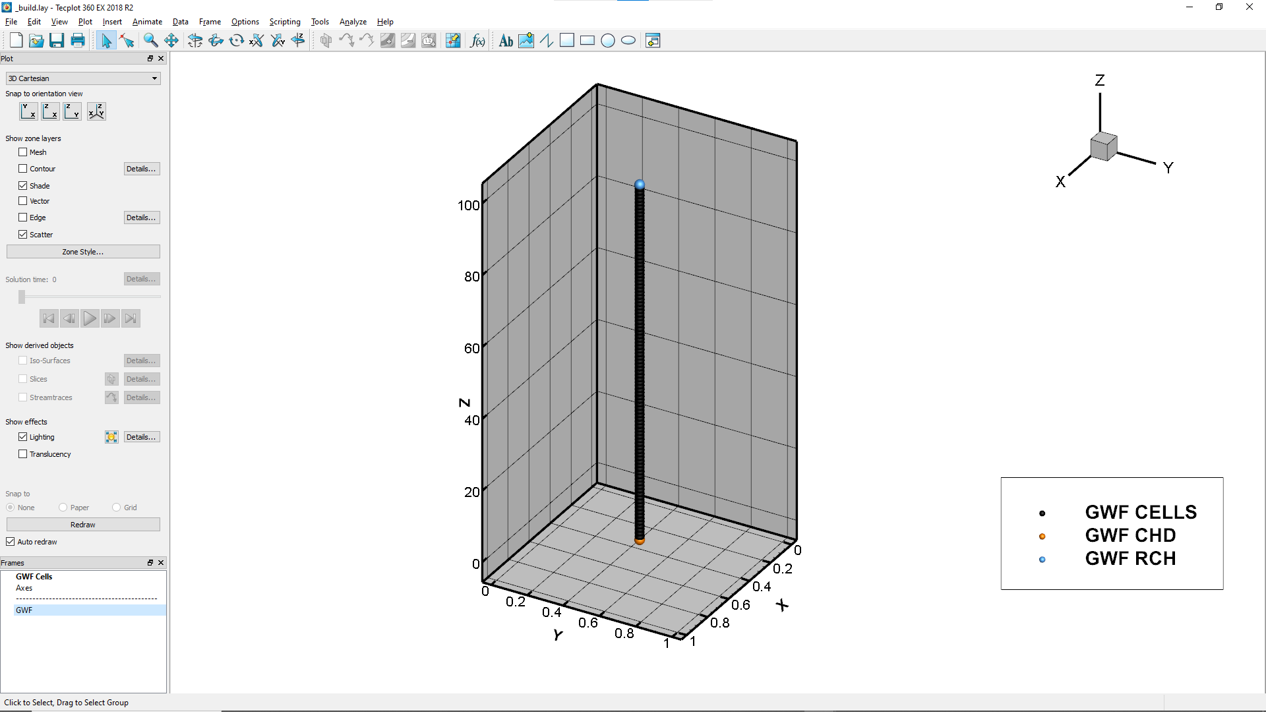
\includegraphics[width=\textwidth]{3_22_GWF_Cells}


\index{\gwf\ Domain ! {\tt \_build.lay} ! {\sf GWF Cells} frame}
The {\sf GWF Cells} frame has the following contents:
\begin{itemize}
  \item The legend, which shows three types of scatter points called {\sf GWF Cells, GWF CHD} and {\sf GWF RCH}, is shown at the middle right side.
   \item The \mfus\ cell locations are shown by the black spheres.
   \item The cell assigned recharge is shown by the large blue sphere.
   \item The cell assigned a constant head is shown by the large green sphere.
\end{itemize}

If boundary conditions are assigned to the \gwf\ domain, as they are in this case, then Tecplot output files will be produced for each type.  The {\tt \_build.lay} file has been configured to load these files.

       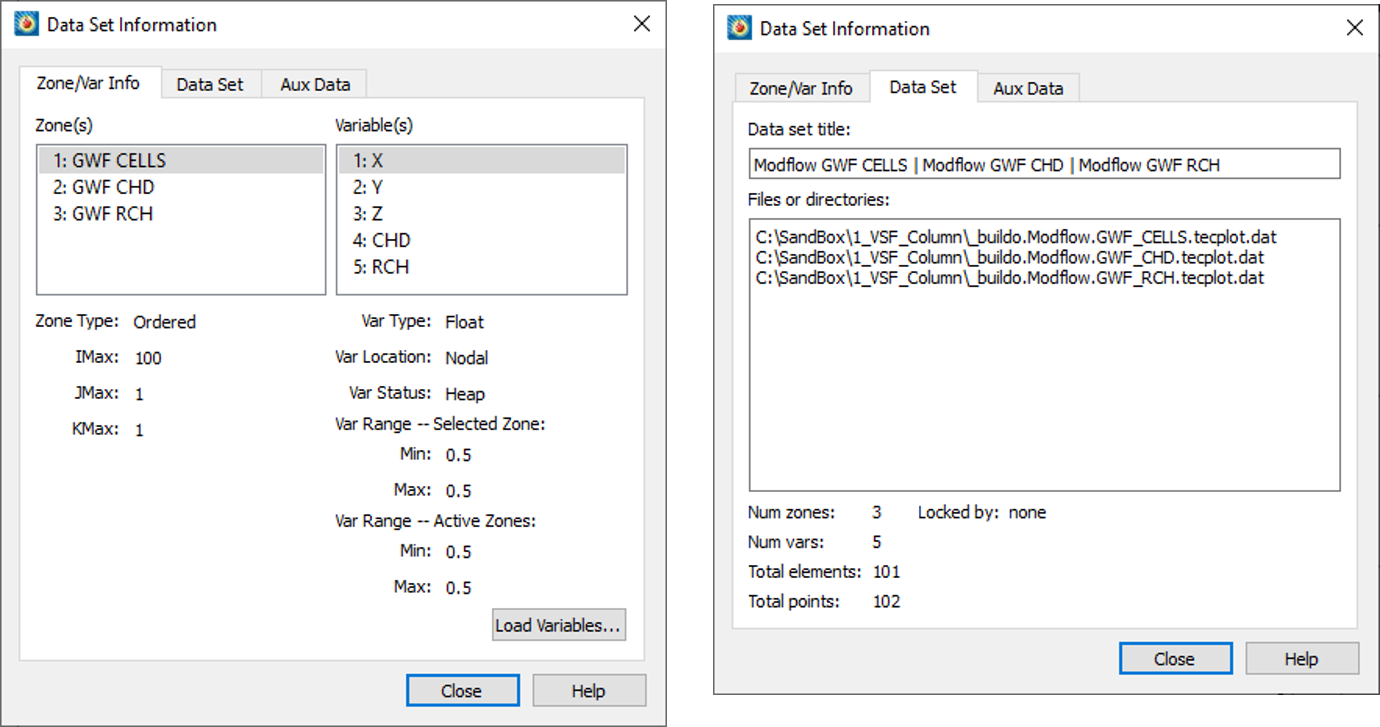
\includegraphics[width=.75\textwidth]{3_23_GWF_CellsDataInfo}

In the {\sf Zone/Var Info} tab, there are 3 zones, and 5 variables.  In the {\sf data Set} tab, we can see that 3 files have been loaded.  

Try to probe the blue sphere, and you will likely get the following warning:

       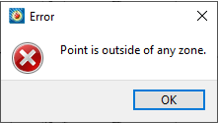
\includegraphics[width=.25\textwidth]{3_24_GWF_CellsPointOutside}

This is because the cell is located at an exact $XYZ$ point, and the chance of clicking the mouse right there is very small.  In this case, to obtain {\it exact} values for the data point nearest the specified location, hold down the {\sf Control} key while clicking the mouse at the desired location.

       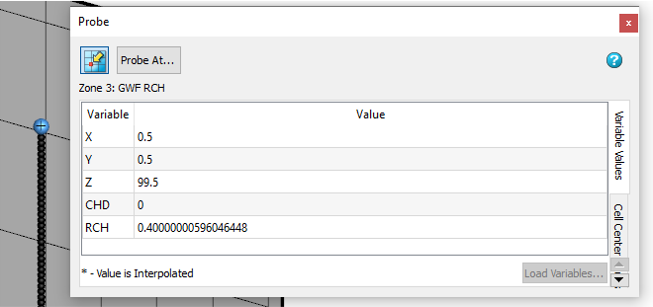
\includegraphics[width=.5\textwidth]{3_25_GWF_CellsControlClick}

You must make sure to have the {\sf Variable Values} tab selected to see values. Here, we see the $XYZ$ location of the nearest cell, and the recharge ({\sf RCH}) value 0.4.  Note that the {\sf CHD} value of 0 is shown by default at non-constant head nodes, and does not mean a constant head of zero has been assigned.   If we probe the probe the green sphere we see this. 

       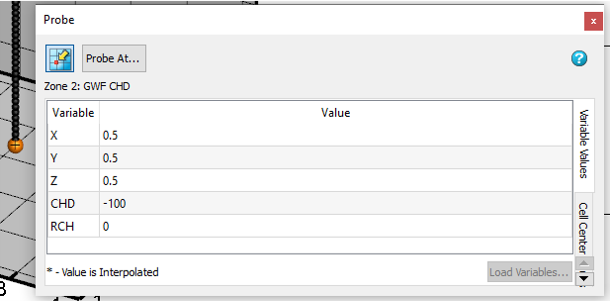
\includegraphics[width=.5\textwidth]{3_25b_GWF_CellsControlClick}

Now the constant head ({\sf CHD}) value -100 is shown while the {\sf RCH}) value is 0, because this is not an assigned recharge cell.

Since this verification example is using mesh-centred control volumes, the cells are located at the center of the finite element prisms.

The verification example \texttt{6\_Abdul\_Prism\_Cell} has a \swf\ domain defined by an irregular 2D surface with a recharge boundary condition assigned to the entire domain and a critical depth outflow boundary condition assigned at the downstream outlet. Since it also has a \gwf\ domain the {\sf \_build.lay} file is a bit more complicated, but has many of the previous example. 

Start a new command prompt, run \tecplot\ and load the {\sf \_build.lay} file.

        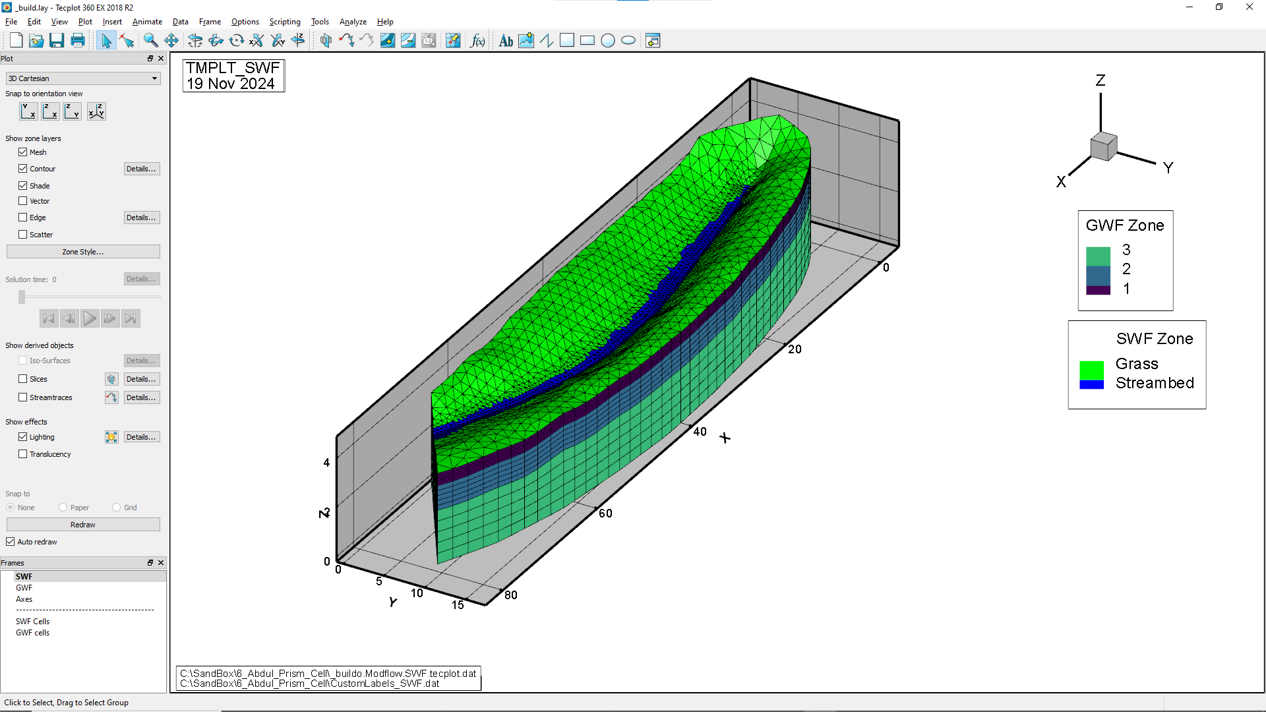
\includegraphics[width=\textwidth]{3_26_SWF_GWF}
        
Here we can see the {\sf SWF, GWF} and {\sf Axes} frames are visible (i.e. placed above the {\sf background} frame in the list).  The {\sf SWF} is currently active (i.e. the name is bolded) and placed at the front of the image (i.e. at the top of the list). It uses a different colormap to make it easier to distinguish the \gwf\ domain below.  

Send the {\sf GWF} and {\sf Axes} frames to the back to see only the contents of the {\sf SWF} frame.

        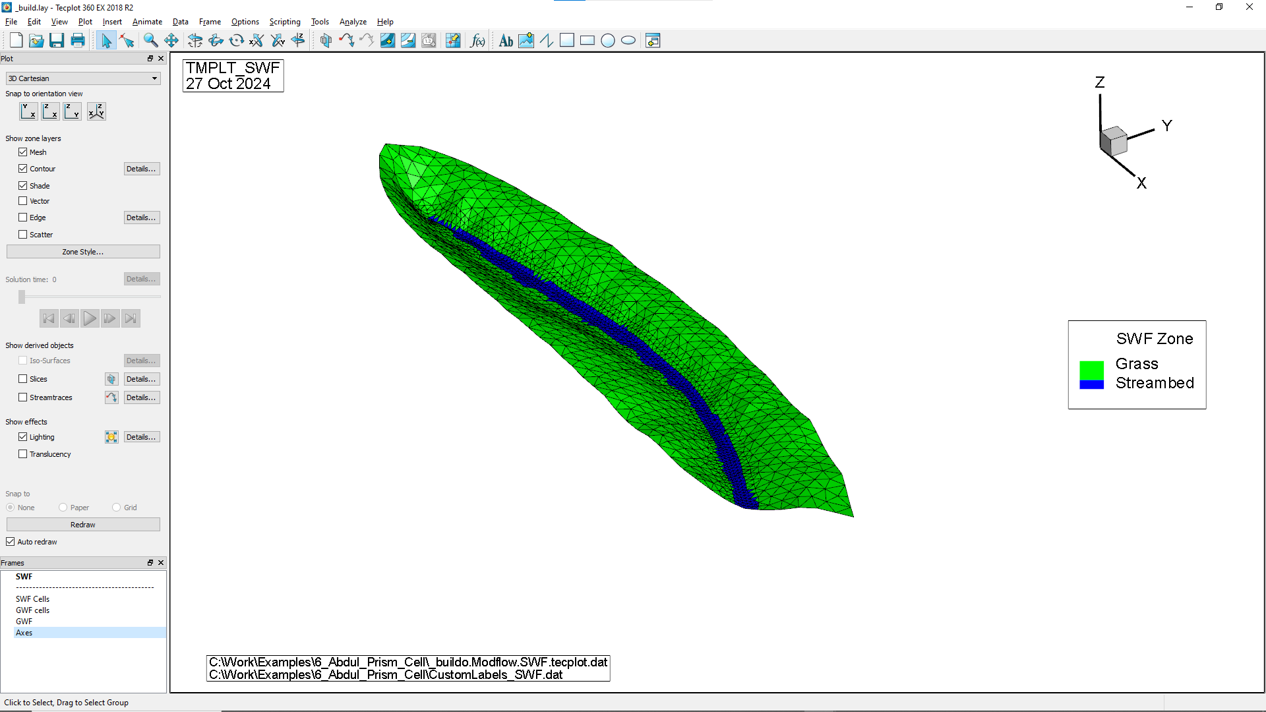
\includegraphics[width=\textwidth]{3_27_SWF}
        


\index{\swf\ Domain ! {\tt \_build.lay} ! {\sf SWF} frame}
The {\sf SWF} frame has very similar contents to the {\sf GWF} frame described earlier, but note that:
\begin{itemize}
  \item The names of the data files loaded into the frame are for the \swf\ domain.
  \item   The data set title {\sf TMPLT\_SWF} indicates that this is the \swf\ domain mesh that was created from the template mesh.
  \item The contouring legend, showing there are two \swf\ zones called {\sf Grass} and {\sf Streambed} is a bit more descriptive than e.g. {\sf Zone 1}.   These are referred to a custom labels in \tecplot.
\end{itemize}

\index{\tecplot\ ! custom labels} To define custom labels as shown for the \swf\ legend, and earlier for the \gwf\ legend, you must define a tecplot file that contains the custom label set.  This is in fact the second file loaded in the \swf\ frame called {\tt CustomLabels_SWF.dat}.  It looks like this:
\begin{verbatim}
    CUSTOMLABELS
    "Streambed",
    "Grass",
    "Zone 3",
    "Zone 4",
    "Zone 5",
    "Zone 6",
\end{verbatim}

        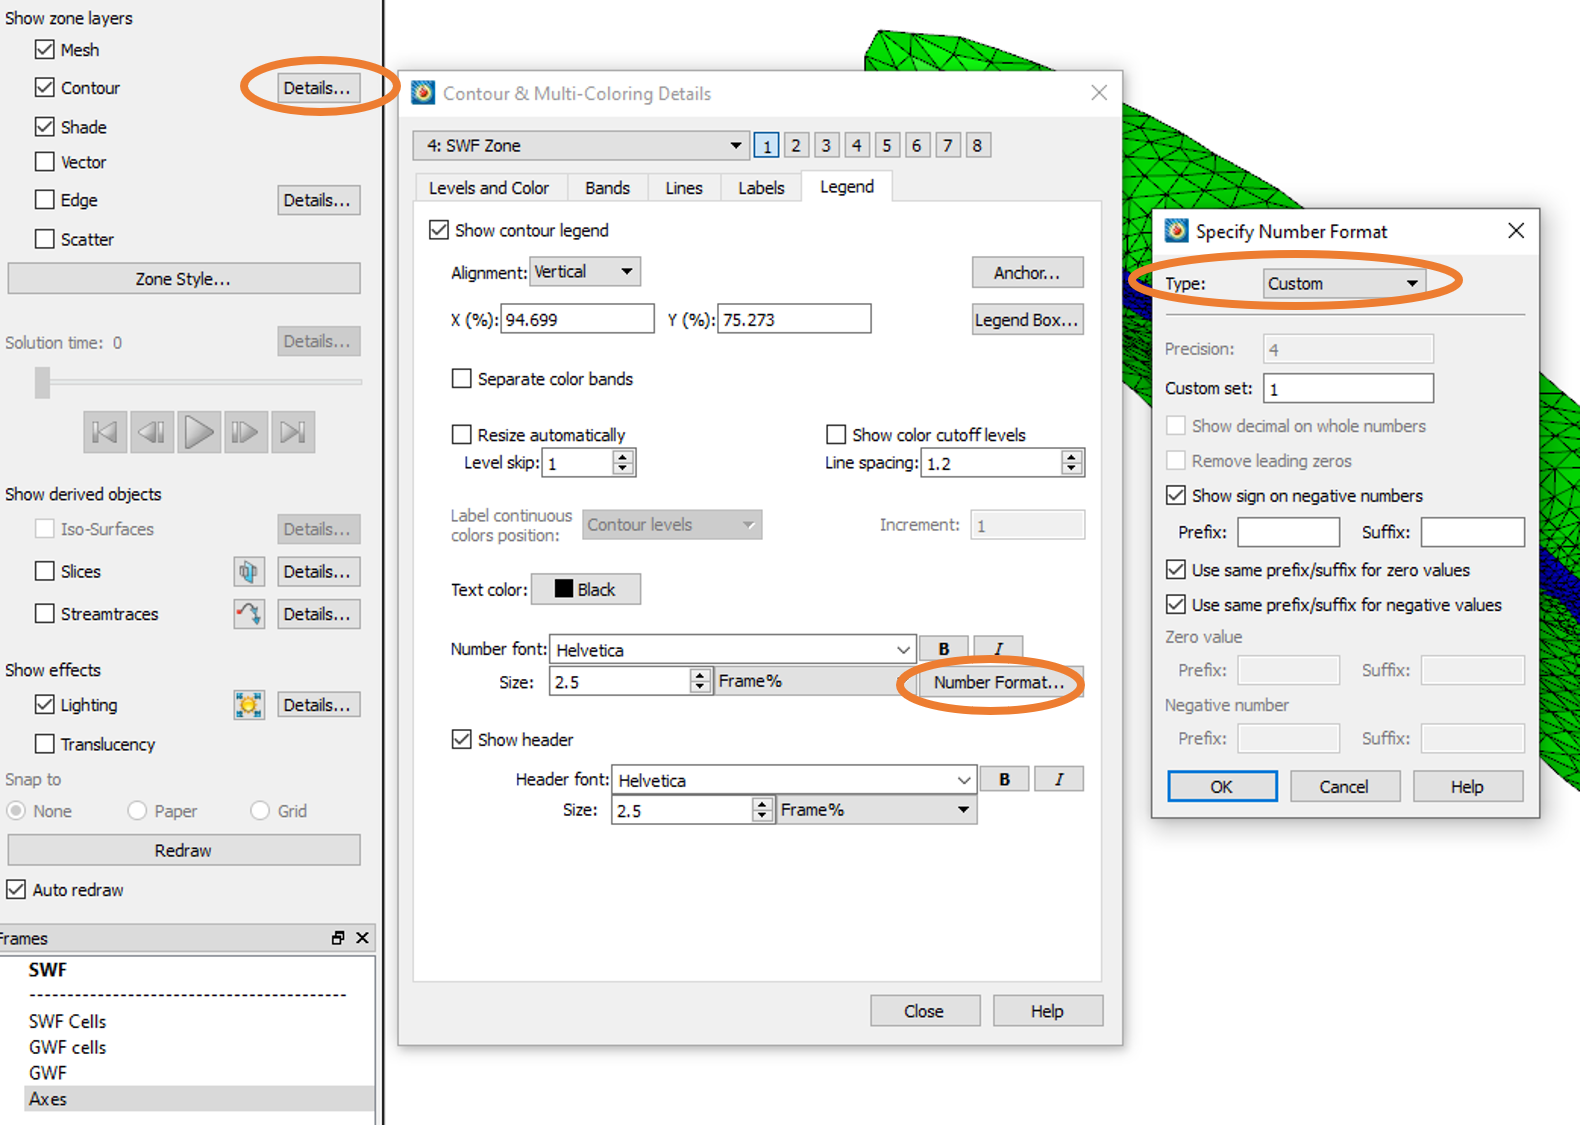
\includegraphics[width=\textwidth]{3_28_SWFCustomLabels}
        
The use of custom labels is configured by first choosing the contouring {\sf Details...} button, which opens the {\sf Contour & Multi-Coloring Details} dialogue.  Choose the {\sf Number Format...} button to open the {\sf Specify Number Format} dialogue, then choose {\sf Custom} from the {\sf Type:} drop-down menu. 
